\section{Cronograma}
\label{sec:cronograma}

O cronograma do projeto, dividido em 12 meses, é apresentado na Figura \ref{fig:cronograma}.

\begin{figure}[H]
    \caption{Cronograma do projeto.}
    \label{fig:cronograma}
    \centering
    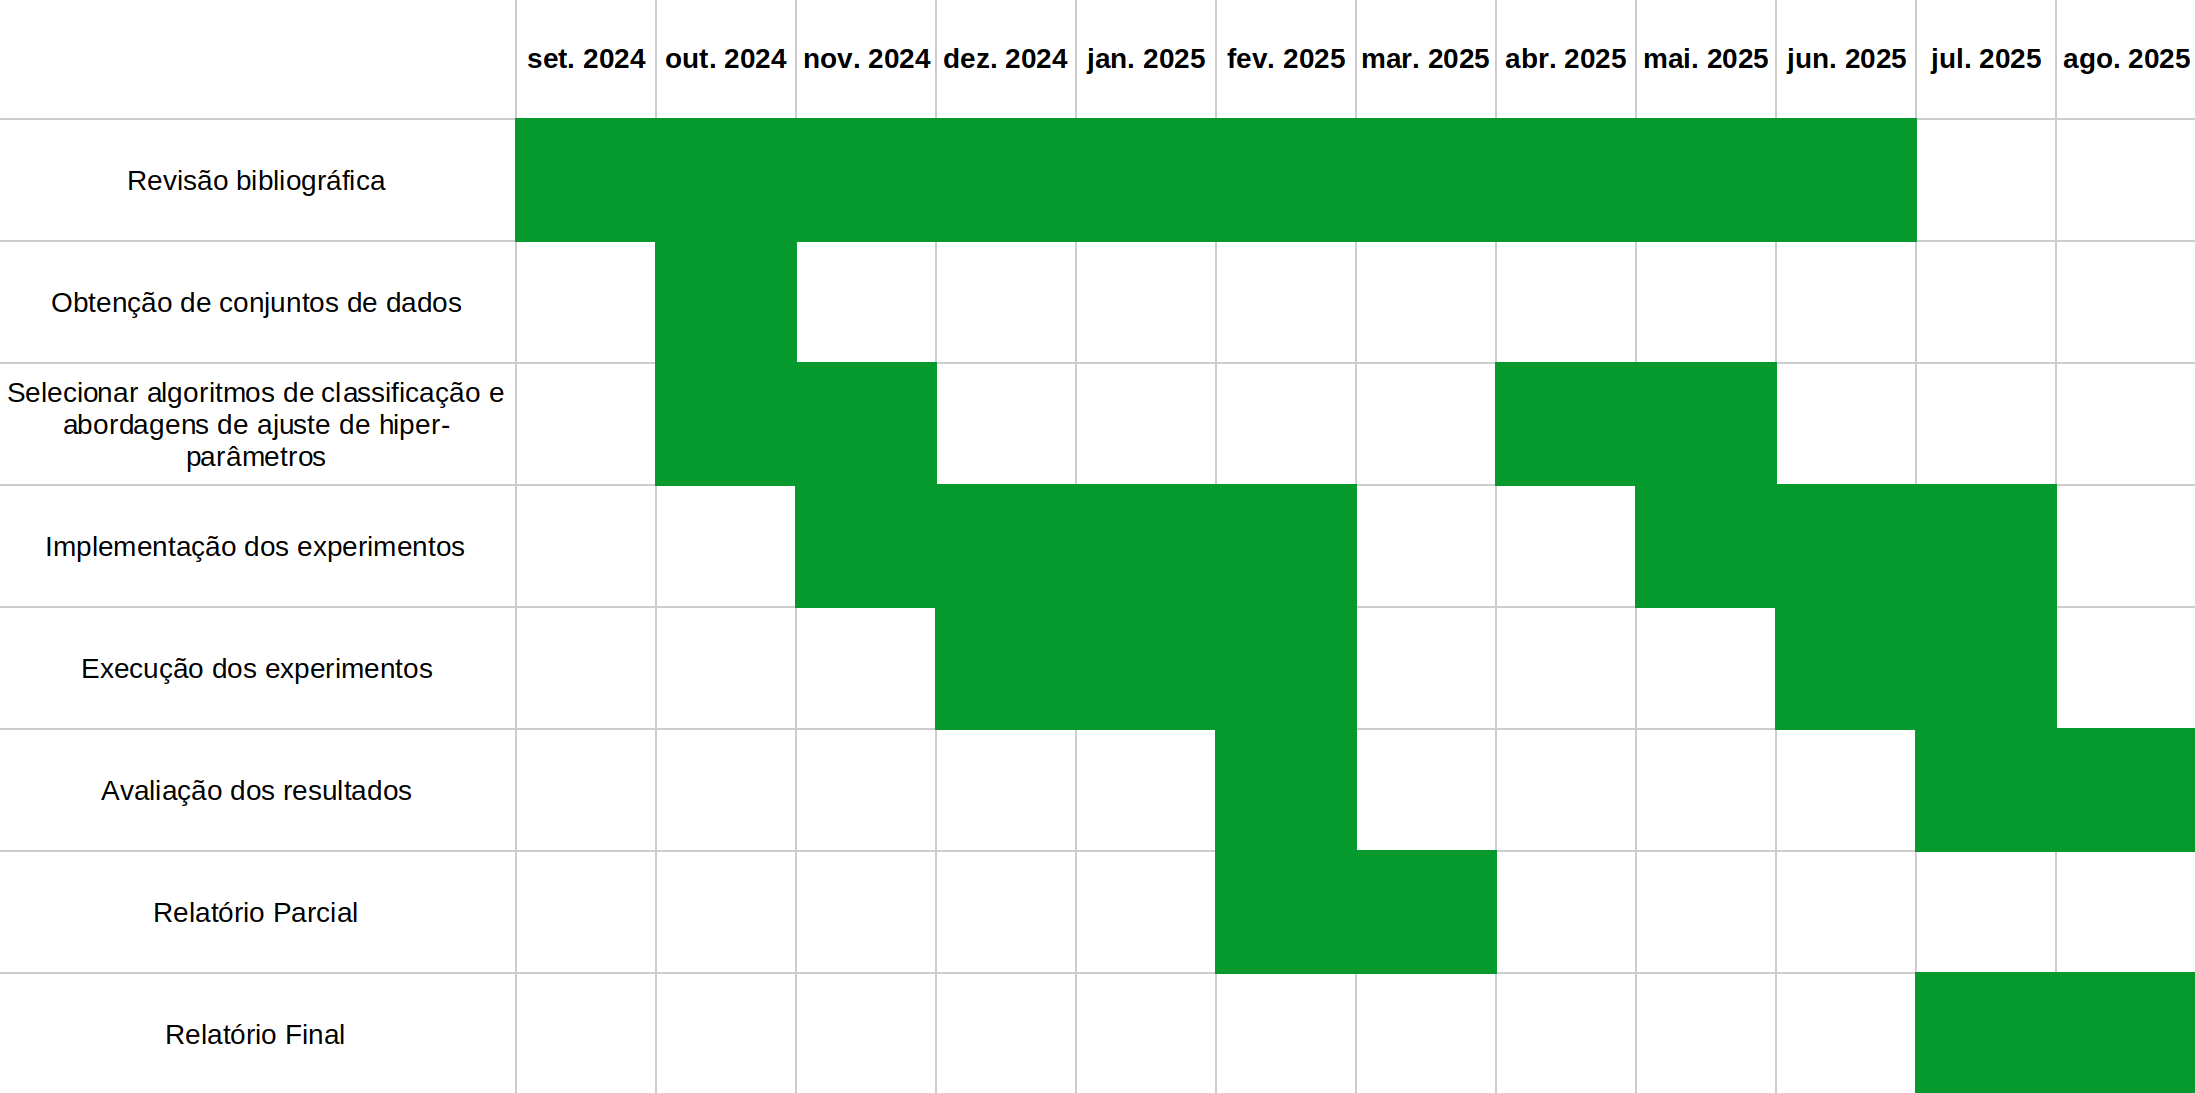
\includegraphics[width=\textwidth]{cronograma.png}    
\end{figure}

As tarefas do cronograma são brevemente descritas a seguir:

\begin{itemize}
    \item \textit{Revisão bibliográfica}: pesquisa de trabalhos relacionados a dinâmica da digitação e ajuste de hiperparâmetros;
    \item \textit{Selecionar algoritmos de classificação e abordagens de ajuste de hiperparâmetros}: definir quais algoritmos de aprendizado de máquina serão utilizados na classificação dos dados de dinâmica da digitação, assim como as abordagens de ajuste de hiperparâmetros que serão avaliadas;
    \item \textit{Obtenção de conjuntos de dados}: obtenção de conjuntos de dados para os experimentos. Alguns conjuntos de dados que podem ser utilizados são mencionados na Sessão~\ref{sec:datasets};
    \item \textit{Implementação dos experimentos}: implementação do código para realizar os experimentos;
    \item \textit{Execução dos experimentos}: execução dos experimentos com diferentes abordagens de ajuste de hiperparâmetros;
    \item \textit{Avaliação dos resultados}: avaliação dos resultados obtidos nos experimentos;
    \item \textit{Relatório Parcial}: elaboração do relatório parcial;
    \item \textit{Relatório Final}: elaboração do relatório final.
\end{itemize}

Além das atividades descritas no cronograma, artigos científicos poderão ser escritos e submetidos.